%!TEX TS-program = xelatex
%!TEX encoding = UTF-8 Unicode

\documentclass[11pt,tikz,border=1]{standalone}
\usetikzlibrary{positioning}

\begin{document}
  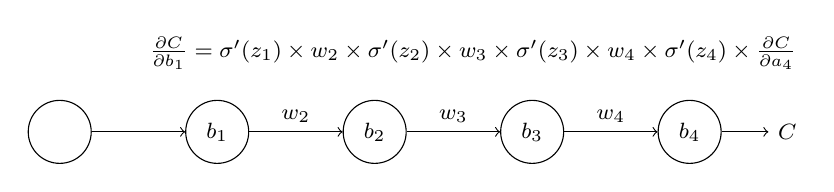
\begin{tikzpicture}[
    neuron/.style={circle,draw,inner sep=0pt,minimum size=8mm},
    font=\footnotesize
    ]

    \node (b0) [neuron] {};
    
    \foreach \x in {1,...,4}
      \node (b\x) [neuron] at (\x * 2, 0) {$b_{\x}$};

    \draw[->] (b0) -- node [above] {} (b1);
    \draw[->] (b1) -- node [above] {$w_2$} (b2);
    \draw[->] (b2) -- node [above] {$w_3$} (b3);
    \draw[->] (b3) -- node [above] {$w_4$} (b4);
    \draw[->] (b4) -- ++(1,0) node (c) [right] {$C$};

    \node[above=1,anchor=east] at (c.east) {
      $\frac{\partial C}{\partial b_1} = \sigma'(z_1) \times w_2 \times \sigma'(z_2) \times w_3 \times \sigma'(z_3) \times w_4 \times \sigma'(z_4) \times \frac{\partial C}{\partial a_4}$
    };

  \end{tikzpicture} 
\end{document}
